% !TEX root = BachelorBookletMain.tex

\chapter{Workflow}
In this project I fallowed an iterative prototype workflow creating a prototype to evaluate a specific ideas. As for implementing different systems needed for the prototype I followed the workflow of researching a single component\footnote{such as the Kears functional API, UDP sockets, etc.} and implementing it, before beginning further researching efforts.

What fallows is a description of the prototypes developed over the course of the project. The main prototype "maze game" was the main focus of the project after the direction of the project was defined using the results from previous prototypes as guidance. It is described in detail in \cref{MazeGameSystems}.


\subsection{Functional}
The first prototype was developed with the intension of establishing the core systems. The entire data generation- and preprocessing pipeline and the neural network model where implemented and evaluated. A small level with checkerboard textures, seen in \cref{Functional}, and variable sky and wall colors between environments was created to evaluate the systems. \todo{make a distinction between environment and level everywhere in the document, where environment is a variation of a level}

\begin{figure}[p]
  \centering
  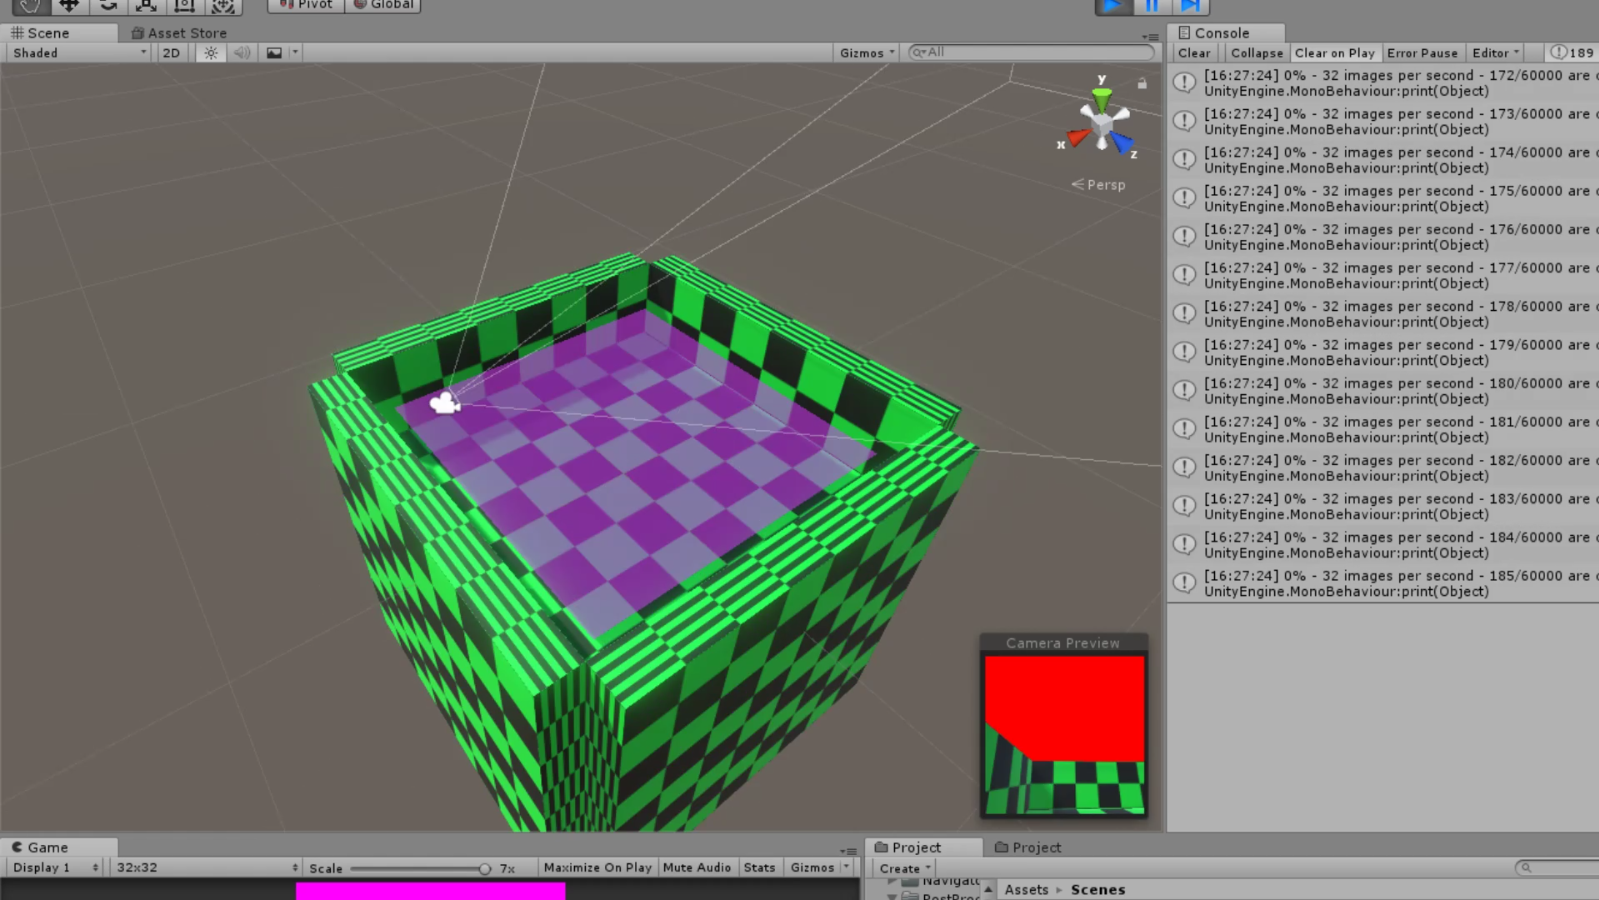
\includegraphics[width=\imgWidth]{images/workflow/Functional1.png} \\[\picVdist]
  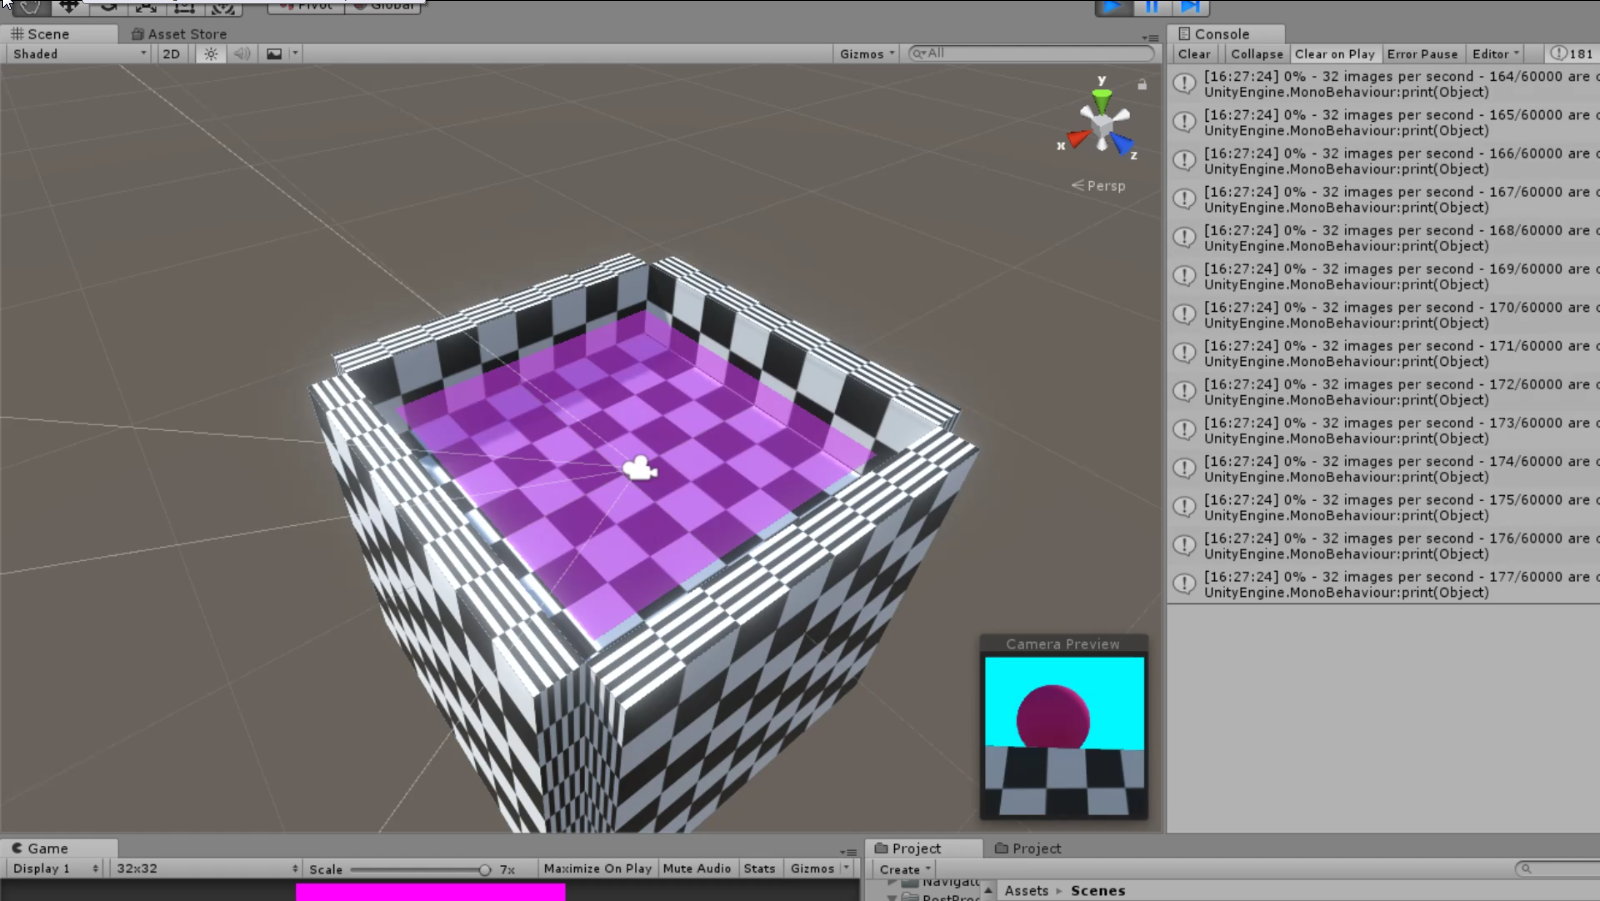
\includegraphics[width=\imgWidth]{images/workflow/Functional2.png}
  \caption{The environment of the functional prototype}
  \label{Funcional}
\end{figure}


\subsection{Top down}
This prototype was used to evaluate the suitability of the network for a top town game. In this prototype the player is supposed to go from one colored platform to another while avoiding running into red walls. The challenge should be created by only training the network on data captured when the camera points at one of the colored platforms. Training the network on this data resulted only in making the network output blurry, when the player was not positioned on a platform (see \cref{WalkOffPlatform}).

\begin{figure}[p]
  \centering
  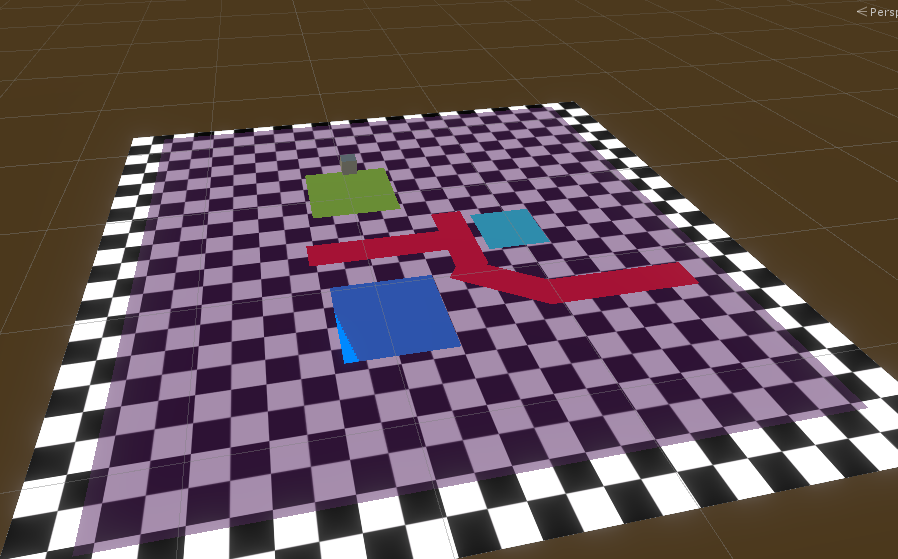
\includegraphics[width=\imgWidth]{images/workflow/TopDownLevel.png}
  \caption{Top down level as seen in the editor}
  \label{TopDownUnity}
\end{figure}

\begin{figure}[p]
  \centering
  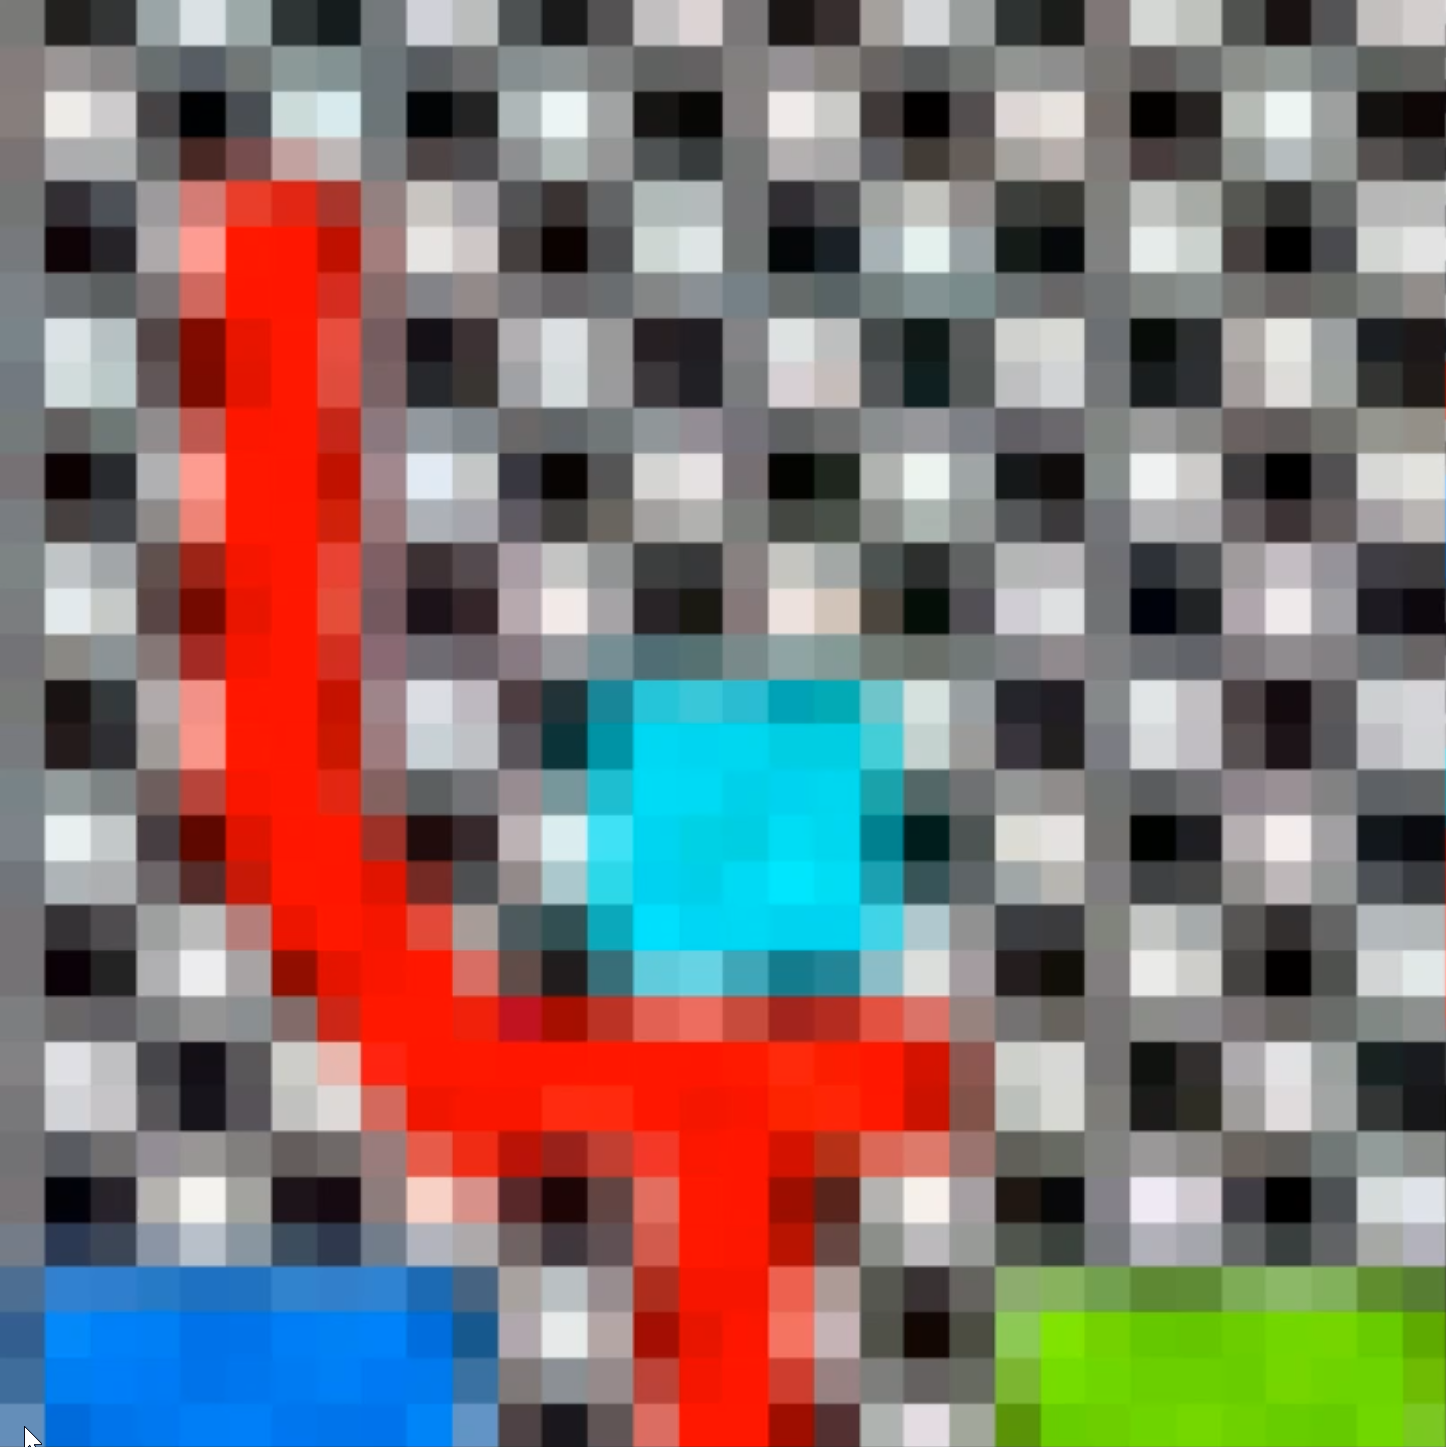
\includegraphics[width=\imgWidth]{images/workflow/TopDownOn.png} \\[\picVdist]
  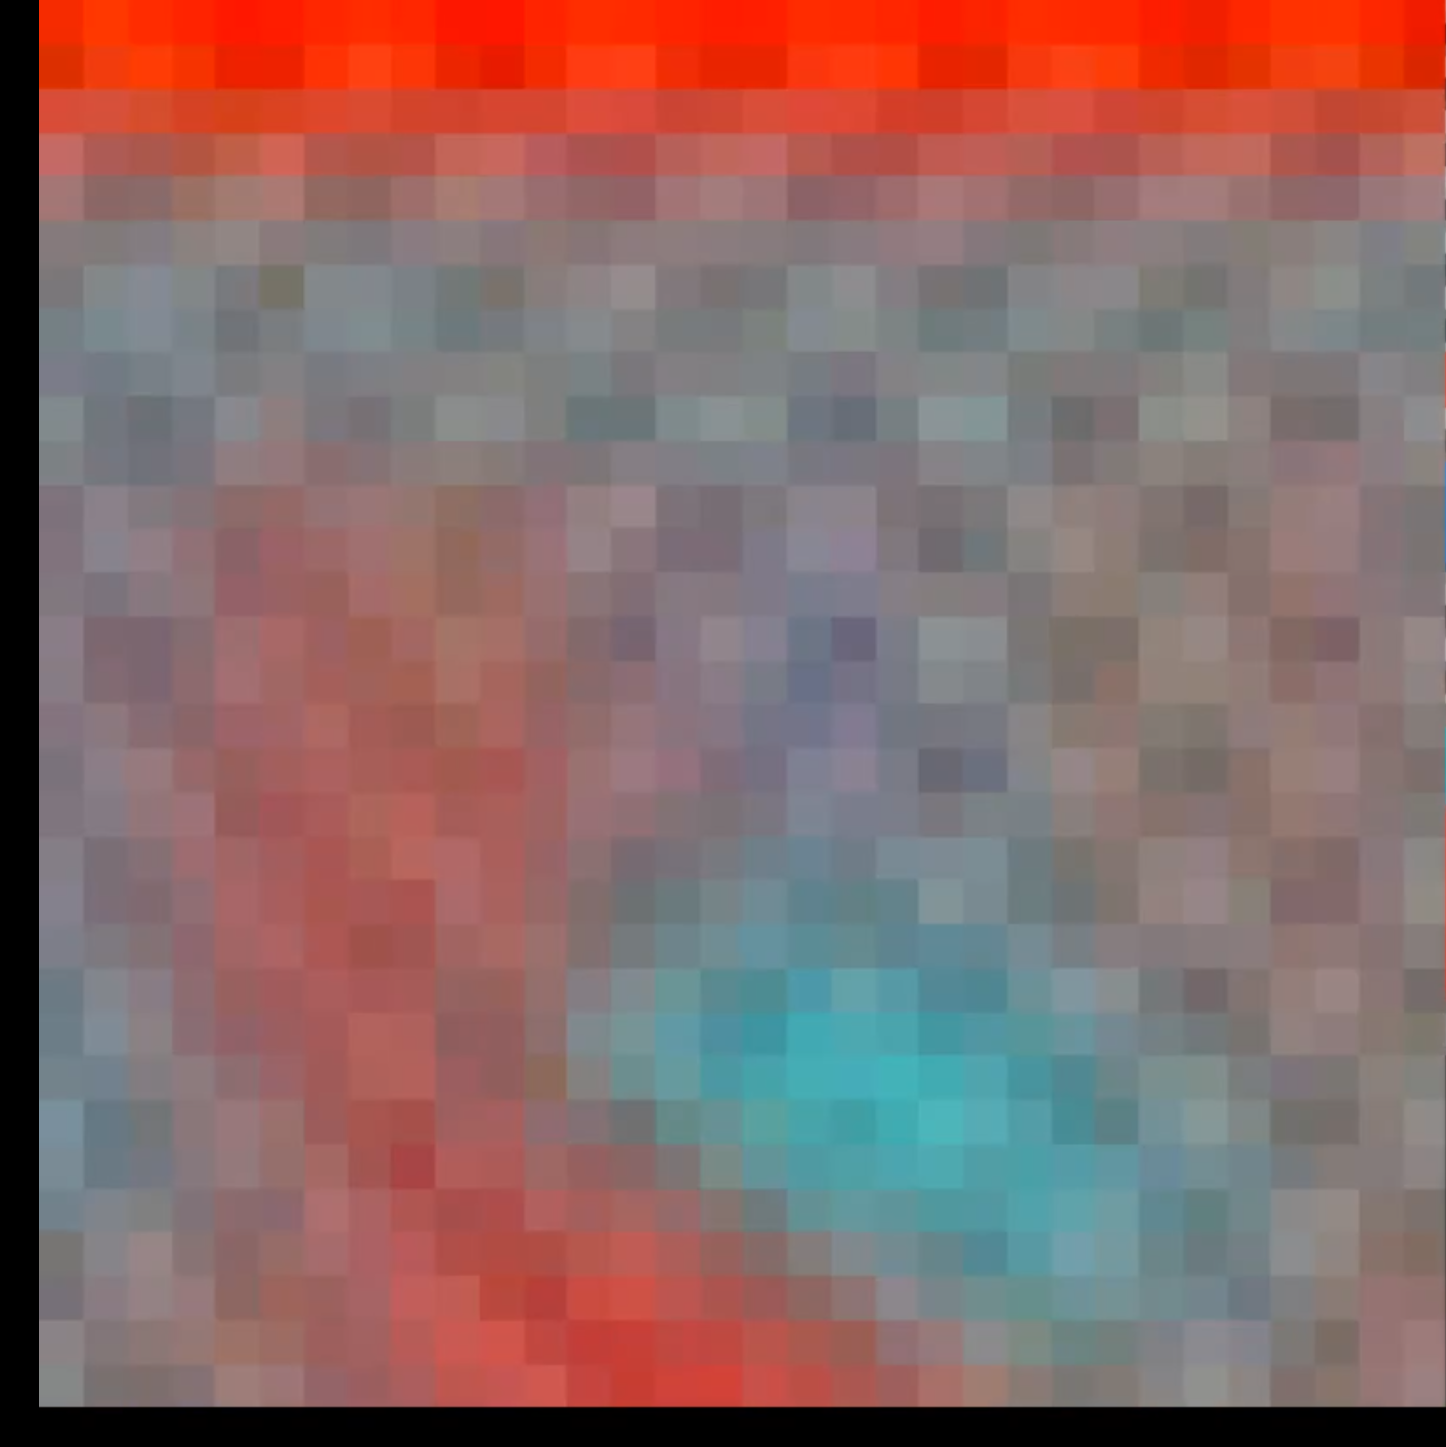
\includegraphics[width=\imgWidth]{images/workflow/TopDownOff.png}
  \caption{The network output gets blurry when the player walks off a platform.}
  \label{WalkOffPlatform}
\end{figure}


\subsection{Walking sim}
Here the idea was to use the neural network to present the environment to the player through the neural network to create an interesting visual appearance. It also was experimented with having certain objects only be visible if the player is a certain position in the environment (see \cref{WalkingSim}). This idea was further explored in the next prototype.

\begin{figure}[p]
  \centering
  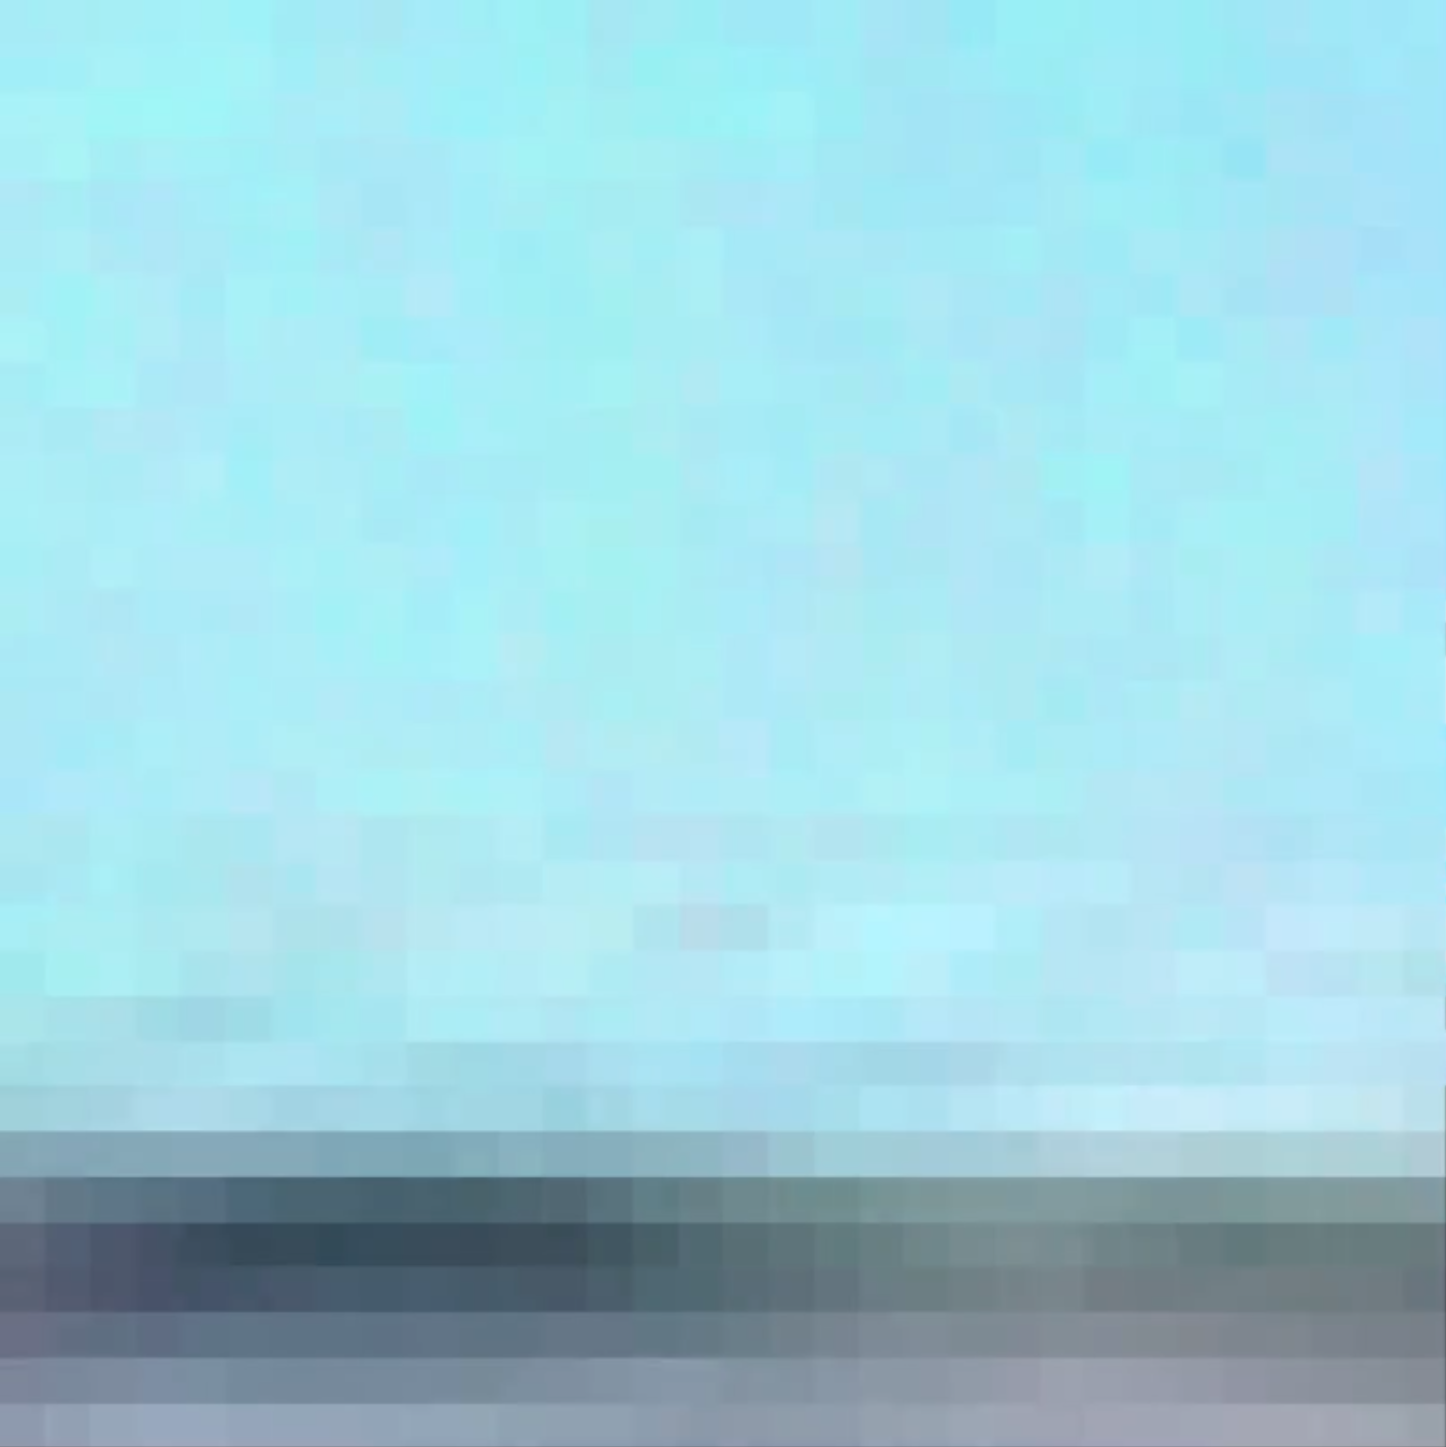
\includegraphics[width=\imgWidth]{images/workflow/WalkingSimNothing.png} \\[\picVdist]
  \includegraphics[width=\imgWidth]{images/workflow/WalkingSimClound.png}
  \caption{Objects can only be seen, when the player stands at certain locations}
  \label{WalkingSim}
\end{figure}


\subsection{Object morphing}
This prototype has a level that is divided into four differently colored platforms that are surrounded by tall pillars. The pillars and the coloring of the platforms help the player to orient himself. In the center four different objects are placed. Each of the object is linked with a different marker group as described in \cref{DataGeneration}. There is maker placed for each platform. This means that if an observation is taken from a specific platform only one object is displayed in the center. When the player crosses from one platform to another the center object is morphed from one object to another in an interpolated way. This is because if a network has a limited amount of parameters it can not model an instantaneous change in "pixel space".

\dl{cimg('picture without object')}
\dl{cimg('img of the morphing center object')}

\dl{cimg('img of the morphing center object')}

\dl{cimg('img of unity scene')}
